\documentclass[twocolumn,a4j]{jarticle}
\documentclass[titlepage]{jarticle}
\usepackage[dvipdfmx]{graphicx}
\usepackage[dvipsnames]{xcolor}
\usepackage{float}
\usepackage{array}
\usepackage{colortbl}
\usepackage{tabularx}
\usepackage{multirow}
\newcolumntype{C}{>{\centering\arraybackslash}X} %中央揃え
\newcolumntype{R}{>{\raggedleft\arraybackslash}X} %右揃え
\usepackage{afterpage}
\graphicspath{{eps/}}
\textwidth=150mm
\textheight=237mm
\usepackage{geometry}
\geometry{left=30mm,right=30mm,top=30mm,bottom=30mm}

\makeatletter
\renewcommand{\theequation}{% 式番号の付け方
\thesection.\arabic{equation}}
\@addtoreset{equation}{section}
\renewcommand{\thefigure}{% 図番号の付け方
\thesection.\arabic{figure}}
\@addtoreset{figure}{section}
\renewcommand{\thetable}{% 表番号の付け方
\thesection.\arabic{table}}
\@addtoreset{table}{section}
\makeatother
%%
%%
%% 以下のスタイル情報は変更しない
\setlength{\textheight}{277mm}
\setlength{\textwidth}{180mm}
\setlength{\topmargin}{-35mm}
\setlength{\oddsidemargin}{-9mm}

\usepackage{secdot}
\sectiondot{subsection}

%%
%% 
%% 論文タイトルを記入
\title{
  感情表現の訓練を目的とした人とロボットのインタラクション
}   

%%
%% 
%% 氏名、学籍番号、指導教員を記入
\author{
  佐賀大学 理工学部 理工学科 知能情報システム工学コース\\
   発表者:明石 華実 (19238901)\\
  指導教員:福田 修 教授,Yeoh Wen Liang プロジェクト助教
}


\begin{document}
\date{\empty}
\maketitle
\thispagestyle{empty}

%%
%%
%% section や subsection を必要に応じて用い、本文を記述する。

%%--------------------------------------------------------------------------------
\section{はじめに}
\vspace{-2mm}
%感情を解読した結果,期待される反応や行動のフィードバックを得られると,コミュニケーションやインタラクションの満足度が上がる.これにより,我々は他者とより親密な関係になり,心の通うコミュニケーションを構築し,円滑な人間関係を維持することを実現していると考える.しかしながら,感情の解読を的確に行うことは思いの外困難であるとされている\cite{endo}.

%【表情表出の訓練への期待】
%感情表出のトレーニングを通して,感情の表出を適切に行うことで,表情の解読をより的確に行うことが期待されている.しかしながら,感情表出トレーニングの難しさも数多く指摘されている.表情を表出するトレーニングは,鏡や対人での実施が最も一般的であるが,「客観的なフィードバックを得られない」や「緊張感を覚えたり,気軽さに欠けたりする」といった問題が考えられる.また,外部からの日々のタスクとして支持されるトレーニングは,利用者の負担になり,継続率が低下すると考える.

%【ロボットを利用した表情表出の訓練の提案】
%そこで,本研究では,表情を表出するトレーニングを日常的に行うことを目的として,感情表現に基づき人とインタラクションするロボットの開発を目標とする.ロボットなどのエージェントを用いることで,利用者の負担軽減と継続率低下の抑制も期待され,ロボットとのコミュニケーションを円滑に行えるようになることで,効果を実感する機会を増やし,継続率低下を抑制できると考えられる.
円滑な感情の表出や読解はコミュニケーションやインタラクションの満足度につながる.しかし,感情表出を適切に行うことができず,他者の感情を的確に理解することが困難な場合もある\cite{sato}.
そこで,本研究では,表情表出トレーニングを目的とし,感情表現に基づいて人とインタラクションするロボットの開発を目標とする.エージェントを用いることで利用者に負担をかけずに円滑なコミュニケーションを実現し,効果を実感させる機会を与え,継続率低下の抑制を目指す.


%%--------------------------------------------------------------------------------
\vspace{-4mm}
\section{システム概要}
\vspace{-2mm}
システムの概要を図\ref{System Overview}に示す.システムは,カメラ(Logicool C922n)から得られる動画像から,クラウドプラットフォーム(Amazon Web Services)を利用して感情推定を行い,その推定結果に基づいて,ワンボードマイコン(Rasberry Pi 3 Model B)で,ロボットのサーボモータ(KeiganMotor KM-1S)を制御する.図\ref{System Overview}で示すように,Motor 1は尻尾の左右運動,Motor 2は上下運動を制御する.
%%-------------------------------------------------------------------------------
\vspace{-2mm}
\begin{figure}[h]
\begin{center}
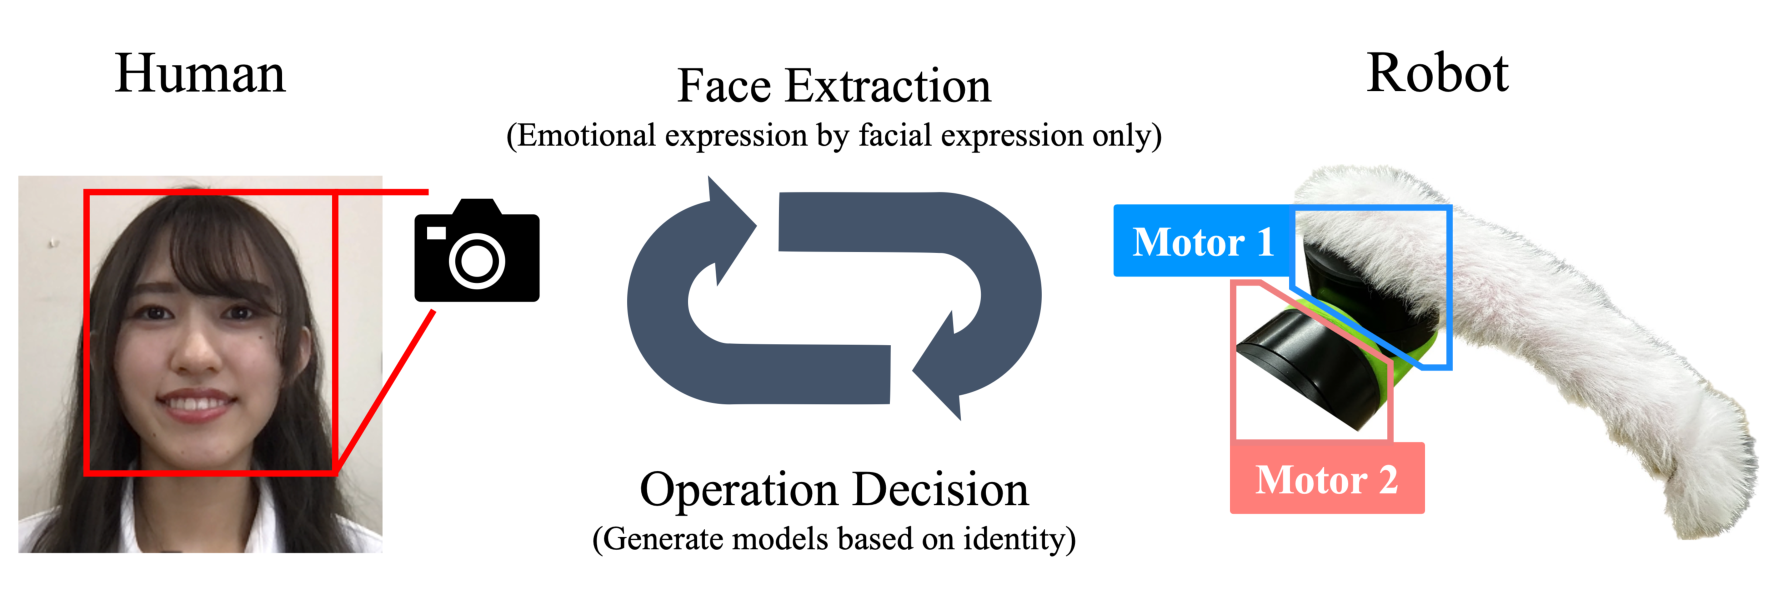
\includegraphics[scale=0.21]{System_over_new.eps}
\end{center}
\vspace{-8mm}
\caption{システム概要}
\label{System Overview} %ここでは図のラベルを指定できます。詳しくはこの後記述します。
\end{figure}
%%--------------------------------------------------------------------------------
\vspace{-8mm}
\section{トレーニングの効果の検証実験}
\vspace{-2mm}
感情に基づいて行動するロボットを用いたトレーニングを実施し,表現力向上の効果と,心理的な効果について検証を行った.

被験者は20代男女10名とした.被験者は,各々表情表出トレーニングを5分間行う.トレーニングの前後では,指定される感情を5秒間,表情のみで表現する.指定される感情は,「$\rm\,I\,$:HAPPY」,「$\rm\,II\,$:ANGRY」,「$\rm\,III\,$:SURPRISED」,「$\rm\,IV\,$:SAD」,「$\rm\,
V\,$:CALM」の5種類である.これら5つの各感情をランダムに指定することを1セットとして,トレーニングの前後で,2セットずつ行った.被験者がトレーニングを行う際のフィードバックの方法は,「(A):鏡」と「(B):ロボット」の2種類とした.また,被験者に実験の前後に心理状態などを調査するアンケート調査を実施した\cite{hayashi}.

被験者に指定した感情と,推定結果が一致した割合を正解率とする.(A)での正解率は,Beforeが62.6$%$,Afterが64.0$%$であり,大きな差異はなかった.一方,(B)での正解率は,Beforeが68.0$%$,Afterが77.0$%$であり,9.0$%$上昇した.各条件下でのトレーニング前後では,一部の表情で正解率が上昇したものの,誤った表情をトレーニングしてしまい,正解率が低下した感情もある結果となった.

%また,各条件下でのトレーニング前後でのアンケート調査の結果の平均値を図\ref{Jikken3_Q1}に示す.心理特性において,トレーニング前後での平均値を比較するとBeforeよりAfterの方が,「堅苦しい」などのマイナスな質問項目(Q1,Q2,Q3,Q5)は低下し,「気軽である」などのプラスな質問項目(Q4,Q6,Q7,Q8,Q9,Q10)は上昇した.トレーニング環境での平均値を比較すると鏡でのトレーニング環境よりロボットでのトレーニング環境の方が,トレーニング前後での平均値の比較と同様に,マイナスな質問項目はより一層低下し,プラスな質問項目はより一層上昇した.
また,アンケート調査の結果を図\ref{Jikken3_Q1}に示す.心理状態の調査において,各環境でのトレーニング前後の平均値を比較すると,「Q1:緊張する」,「Q2:堅苦しい」,「Q3:苦手である」,「Q5:疲れる」のネガティブな質問項目は低下し,「Q4:気軽である」,「Q6:孤独を和らげる」,「Q7:楽しい」,「Q8:気軽に心を開ける」,「Q9:集中できる」,「Q10:感情を表現しやすい」のポジティブな質問項目は上昇した.各環境でのトレーニング後の平均値を比較すると(B)の方が,ネガティブな質問項目は低下し,ポジティブな質問項目は上昇した.
また,ロボットでのトレーニング後に,100$%$の人が「表現力が高まったと実感する」と回答し,ロボットでのフィードバックに好意的な意見が多く聞かれた.その一方で,「動作に時差が生じる」などのシステムの問題点も挙げられた.

%図と表%%%%%%%%%%%%%%%%%%%%%%%%%%%%%

%アンケート%%%%
\begin{figure}[h]
\begin{center}
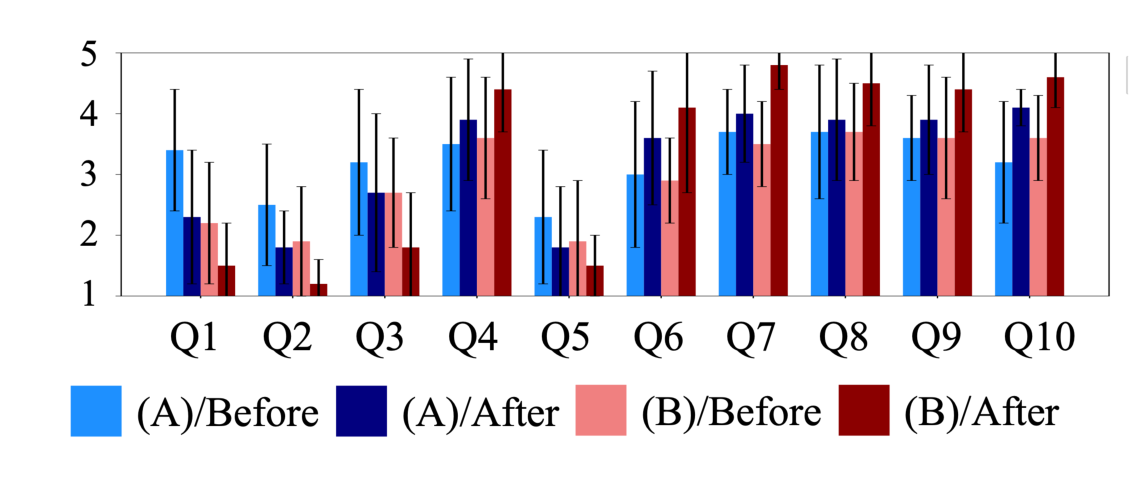
\includegraphics[scale=0.42]{Jikken3_y_q.eps}
\end{center}
\vspace{-8mm}
\caption{心理特性調査}
\label{Jikken3_Q1} %ここでは図のラベルを指定できます。詳しくはこの後記述します。
\end{figure}
\vspace{-9mm}

%%%%%%
\section{まとめ}
\vspace{-2mm}
本研究では,感情表現に基づき人とインタラクションするロボットを開発し,表情を表出するトレーニングを日常的に行うことを目指した.感情推定結果に基づき,行動するロボットの制作と効果の検証を行い,ロボットを用いた表情の表出トレーニングの効果を確認し,表出トレーニングにおいてロボットを用いることの有意性を確認した.今後は,ロボットのフィードバック方法の改良を目標とする.
%%
%%
%% 参考文献を記述する。
\vspace{-9mm}
\begin{thebibliography}{9}\setlength{\itemsep}{-2pt}
%\bibitem{endo}
%遠藤健治, 表情によるコミュニケーション【ススメ!コミュニケーションの新しいカタチ第1回】, 2020,\\
%$https://aogakuplus.jp/column/new_communication_style_20201218_01/$\\
%(参照 2023-01-17)\\
\vspace{-2mm}
\bibitem{sato}
佐藤弥, 嶺本和沙, 吉川左紀子,Facial Expressions of Basic Emotions in Japanese Laypeople, 2019\\
\vspace{-6mm}
\bibitem{hayashi}
林勇吾, Eric, C. , Victor, V. K., 浦尾彰, 小川均, 対話エージェントとのコミュニケーションにおける心理特性 -スキーマと擬人化に関する検討-, 2012\\
\end{thebibliography}
\end{document}